\documentclass{vgtc}                          % final (conference style)

\usepackage{microtype}                 % use micro-typography (slightly more compact, better to read)
\PassOptionsToPackage{warn}{textcomp}  % to address font issues with \textrightarrow
\usepackage{textcomp}                  % use better special symbols
\usepackage{mathptmx}                  % use matching math font
\usepackage{times}                     % we use Times as the main font
\renewcommand*\ttdefault{txtt}         % a nicer typewriter font
\usepackage{cite}                      % needed to automatically sort the references
\usepackage{tabu}                      % only used for the table example
\usepackage{booktabs}                  % only used for the table example

\usepackage{tikz}
\usepackage{tikz-inet}
\usepackage{tikz-3dplot}
\usetikzlibrary{arrows,automata,angles,quotes}
\usetikzlibrary{decorations.markings}
\usepackage{pgf}
\usepgflibrary{shapes.arrows}
\usepackage{color}
\usepackage{makeidx}
\usepackage{amsmath}
\usepackage{amsthm}
\usepackage{amsfonts}
\usepackage{amssymb}
\usepackage{enumerate}

\usepackage[hidelinks]{hyperref}
\usepackage{cleveref}
\usepackage[free-standing-units=true, binary-units=true]{siunitx}
\sisetup{detect-weight=true, detect-family=true, power-font=unit, %mode=text, 
number-math-rm = \ensuremath}
\sisetup{group-digits = integer, group-separator = {\text{\,}},
group-minimum-digits=5}
%\sisetup{round-mode=figures,round-precision=3} %Set the number of default significant figures
\sisetup{round-mode=off,round-precision=3}

\usepackage{xcolor}
% \colorlet{titleColor}{red}

\usepackage{etoolbox}
\usepackage{morewrites}
\usepackage[margin=1in]{geometry}

% \usepackage[protrusion=true,expansion=true]{microtype} 
% \usepackage{mathpazo} % Use the Palatino font

% \usepackage[T1]{fontenc}
% %\usepackage{lmodern}

% \usepackage{graphicx}


% %\usepackage{color}
% \usepackage{makeidx}
\usepackage{amsmath}
\usepackage{amsthm}
\usepackage{amsfonts}
\usepackage{amssymb}
% \usepackage{enumerate}
% %\usepackage{appendix}
% \usepackage{longtable} %Tableau sur plusieurs pages
% \usepackage{multirow}  %Tableau avec plusieurs sous lignes
% \usepackage{ifpdf}
% \usepackage{marginnote}
% %\usepackage{bibunits}
% \usepackage{mathrsfs}
% \usepackage{scalefnt}

%\usepackage[numbers,sort]{natbib}
% \usepackage[backend=biber, style=ieee, citestyle=numeric-comp, natbib=true]{biblatex}
% \addbibresource{biblio.bib}

% \usepackage{multirow}
% \usepackage{epsfig}

% \usepackage[linesnumbered,ruled,vlined,boxed,commentsnumbered]{algorithm2e}
% \usepackage[noend]{algorithmic}
% \usepackage{stfloats}
% \algsetup{linenosize=\tiny}


% \usepackage{newfloat}
% \DeclareFloatingEnvironment[fileext=frm,placement={!ht},name=Frame]{myfloat}
% \usepackage[skip=5pt,font=bf,labelfont=bf]{caption}
% \usepackage{subcaption}
% %\usepackage[caption=false]{subfig}

% \usepackage{wrapfig}
% \usepackage{enumitem}
% \usepackage{url}
% \usepackage{cleveref}

% % tabular
% \usepackage{booktabs}
% \usepackage{tabularx}
% \newcommand\setrow[1]{\gdef\rowmac{#1}#1\ignorespaces}
% \newcommand\clearrow{\global\let\rowmac\relax}
% \clearrow

% tikz and pgfplots
\usepackage{tikz}
\usepackage{tikz-inet}
\usepackage{tikz-3dplot}
\usetikzlibrary{arrows,automata,angles,quotes}
\usepackage{pgf}
\usepackage{pgfplots}
\usepackage{pgfplotstable}
\pgfplotsset{compat=newest}
\usepgfplotslibrary{statistics}
\usepgfplotslibrary{fillbetween}
\usetikzlibrary{shapes,positioning,3d,calc}
\usetikzlibrary{decorations,decorations.pathmorphing,backgrounds,patterns}
\usepgfplotslibrary{groupplots}
\usetikzlibrary{pgfplots.statistics}
\usetikzlibrary{intersections}
\usepgfplotslibrary{units}
\usepgfplotslibrary{external}

\newcommand{\newparag}[1]{\vspace{3pt}\noindent\textbf{#1}.\hspace{3pt}}



% siunit
\usepackage[free-standing-units=true, binary-units=true]{siunitx}
\sisetup{detect-weight=true, detect-family=true, power-font=unit, %mode=text, 
number-math-rm = \ensuremath}
\sisetup{group-digits = integer, group-separator = {\text{\,}},
group-minimum-digits=5}
%\sisetup{round-mode=figures,round-precision=3} %Set the number of default significant figures
\sisetup{round-mode=off,round-precision=3} 

%%\usepackage[nolist]{acronym}
%\usepackage[acronym,automake,toc,nonumberlist,seeautonumberlist]{glossaries-extra}
%\usepackage[acronym,automake,toc, indexonlyfirst]{glossaries-extra}
%\renewcommand{\descriptionlabel}[1]{\hspace*{\labelsep}\textls[80]{\textbf{\scshape{#1}}}}
\usepackage[acronym,automake,nonumberlist]{glossaries-extra}
\usepackage{glossaries-prefix}
%% Define glossary style
\newglossarystyle{mylist}{%
\setglossarystyle{list}% base this style on the list style
\renewcommand*{\glossentry}[2]{%
\item[\glsentryitem{##1}%
\glstarget{##1}{\glossentryname{##1}}]
\glossentrydesc{##1}\glspostdescription}}
%\glossentrydesc{##1}\glspostdescription\space See first p.\space ##2}}

%% Set glossary style
\setglossarystyle{mylist}
%% Create symbol glossary
\newglossary[slg]{symbolslist}{syi}{syg}{Symbolslist}
\glsaddkey{unit}{\glsentrytext{\glslabel}}{\glsentryunit}{\GLsentryunit}{\glsunit}{\Glsunit}{\GLSunit}
\newglossarystyle{symbunitlong}{%
\setglossarystyle{long3col}% base this style on the list style
\renewenvironment{theglossary}{% Change the table type --> 3 columns
  \begin{longtable}{lp{0.6\glsdescwidth}>{\centering\arraybackslash}p{2cm}}}%
  {\end{longtable}}%
%
\renewcommand*{\glossaryheader}{%  Change the table header
  \bfseries Sign & \bfseries Description & \bfseries Unit \\
  \hline
  \endhead}
\renewcommand*{\glossentry}[2]{%  Change the displayed items
\glstarget{##1}{\glossentryname{##1}} %
& \glossentrydesc{##1}% Description
& \glsunit{##1}  \tabularnewline
}
}
\newglossary[flg]{fake}{fls}{flo}{Fake Entries}
%% Make glossary
\makeglossaries

%%Define acro macro
\newcommand\acro[4][\acronymtype]{
    \newglossaryentry{#2glo}{name={#2}, description={#4.}}
    \newglossaryentry{#2}{type=#1, name={#2},
    description={#3.
%    \glsseeformat[See glossary:]{#2glo}
    }, text={#2}, first={#3
    (#2)\glsadd{#2glo}}, plural={#2s}, firstplural={#3s
    (#2s)\glsadd{#2glo}}, long={#3}, longplural={#3s}}
}
\newcommand\acroAlias[3]{%Define an acronym, used to call the gls but always use the full form
    \newglossaryentry{#1}{name={#2}, description={#3.}}
}
%%Define acro macro
\newcommand\acroNoDef[3][\acronymtype]{
    \newglossaryentry{#2}{type=#1, name={#2},
    description={#3.}, text={#2}, first={#3 (#2)}, plural={#2s}, firstplural={#3s
    (#2s)}, long={#3}, longplural={#3s}}
}

%%Define acro for irregular plurials macro
\newcommand\acroPl[6][\acronymtype]{
    %#1 short sing
    %#2 long sing
    %#3 short pl
    %#4 long pl
    %#5 description
    \newglossaryentry{#2glo}{name={#2}, description={#6.}}
    \newglossaryentry{#2}{type=#1, name={#2},
    description={#3.
%    \glsseeformat[See glossary:]{#2glo}
    }, text={#2}, first={#3
    (#2)\glsadd{#2glo}}, plural={#4}, firstplural={#5 (#4)\glsadd{#2glo}}}
}
%%Define symbol macro
\newcommand\acroSymb[3]{%#1 symbol name, #2 description, #3 units
    \newglossaryentry{#1}{type=symbolslist, name={\ensuremath{#1}},
    description={#2.}, text={#2}, unit={#3},}
}
%(#1s)\glsadd{#1glo}}, see=[Glossary:]{#1glo}}}
\newcommand\acroAlwaysShort[2]{
    %#1 short name
    %#2 long name
    \newglossaryentry{#1}{type=fake, name={#1}, description={#2}, text={#1}, first={#1}, plural={#1s}, firstplural={#1s}}
}
\newcommand\acroAlwaysShortWithDef[3]{
    %#1 short name
    %#2 long name
    %#3 description
    \newglossaryentry{#1glo}{name={#1}, description={#3}}
    \newglossaryentry{#1}{type=fake, name={#1}, description={#2. \glsseeformat[See glossary:]{#1glo}}, text={#1}, first={#1\glsadd{#1glo}}, plural={#1s}, firstplural={#1s\glsadd{#1glo}}}
}
\newcommand\acroAlwaysShortNoPlurialWithDef[3]{
    %#1 short name
    %#2 long name
    %#3 description
    \newglossaryentry{#1glo}{name={#1}, description={#3}}
    \newglossaryentry{#1}{type=fake, name={#1}, description={#2. \glsseeformat[See glossary:]{#1glo}}, text={#1}, first={#1\glsadd{#1glo}}, plural={#1}, firstplural={#1\glsadd{#1glo}}}
}
\newcommand\acroShortSurname[2]{\newglossaryentry{#1}{type=fake, name={#2}, description={#2}, text={#2}, first={#2}, plural={#2s}, firstplural={#2s}}}
%%%
\newcommand\ac[1]{\gls{#1}}
\newcommand\acp[1]{\glspl{#1}}
\newcommand\acs[1]{\glsname{#1}}
\newcommand\acl[1]{\glsentrylong{#1}}

%%symbols
%\acroSymb{BSymb}{Average available bandwidth}{\si{Mbit\cdot s^{-1}}}
%%acronyms
\acroNoDef{2D}{two Dimensional}
\acroNoDef{3D}{Three Dimensional}
\acroNoDef{AR}{Augmented Reality}
\acro{ABR}{Adaptive Bit-Rate}{Familly of adaptive streaming protocols which can
ajust the bit-rate of the downloaded video stream to the measured available downloading
bandwidth. Usually the video is available at  multiple bit-rate on the server
and the client decides which representation of the video to download.}
\acroNoDef{AI}{Artificial Intelligence}
\acroNoDef{API}{Application Programming Interface}
\acroNoDef{AQM}{Active Queue Management}
\acro{AOMedia}{Alliance for Open Media}{The Alliance for Open Media s a Joint
Development Foundation Projects. The goal of this non-profit industry consortium
is to develop openn royalty-free standard for multimedia delivery over the
Internet.}
\acro{AVC}{Advanced Video Coding}{Video codec, also denoted as H.264 or
MPEG-4 Part 10, released in September \num{2004}. Even if AVC can support up to
\gls{8K} resolution videos, it was mainly designed to compress videos video with
resolution up to full HD (FHD).}
\acroNoDef{B}{bidirectional-predicted}
\acroNoDef{CDF}{Cumulative Density Function}
\acroNoDef{CDN}{Content Delivery Network}
\acroNoDef{CMSE}{Commulative Mean Square Error}
\acroNoDef{CMT-SCTP}{Concurrent Multipath Transfer SCTP}
\acroNoDef{CPU}{Central Processing Unit}
\acroNoDef{CWND}{Congestion Window}
\acro{DASH}{Dynamic Adaptive Streaming over HTTP}{TODO}
\acroNoDef{DoF}{Degrees of Freedom}
\acroNoDef{E2E}{End-to-end}
\acroNoDef{EPFL}{Ecole Polytechnique F\'{e}d\'{e}rale de Lausanne}
\acroNoDef{FEC}{Forward Error Correction}
\acroNoDef{FIFO}{First-In First-Out}
\acro{FoV}{Field of View}{Angular size of the \gls{viewport}, often expressed as the vertical angular distance and the horizontal angular distance of the \gls{viewport}}
\acroAlias{VAS}{viewport-adaptive streaming}{An extension of \gls{DASH} that takes into account the user's head orientation prediction, in addition to the
prediction of the available bandwidth, to download video segments that maximize the quality in the displayed part of the omnidirectional video}
\acroNoDef{MAE}{Mean Absolute Error}
\acroNoDef{GOP}{Group of Picture}
\acroNoDef{GPS}{Global Positioning System}
\acroNoDef{GPU}{graphics processing unit}
\acroNoDef{GUI}{Graphical User Interface}
\acroNoDef{HAS}{\ac{HTTP} Adaptive Streaming}
\acroNoDef{HLS}{\gls{HTTP} Live Streaming}
\acroNoDef{HDK2}{Hacker Development Kit 2}
\acroNoDef{HDTV}{high definition television}
\acroNoDef{P2P}{Peer-to-Peer}
\acroNoDef{TV}{television}
\acroNoDef{LF}{Light Field}
\acroNoDef{HEVC}{High Efficiency Video Coding}
\acroNoDef{HM-15}{\ac{HEVC} Test Model - 15}
\acroNoDef{HMD}{Head-Mounted Display}
\acroNoDef{HDS}{\gls{HTTP} Dynamic Streaming}
\acroAlwaysShort{HTTP}{Hypertext Transfer Protocol}
\acroAlwaysShort{HTTP/2}{Hypertext Transfer Protocol version 2}
\acroNoDef{I}{intra-predicted}
\acroAlwaysShort{IETF}{Internet Engineering Task Force}
\acroNoDef{ILP}{Integer Linear Program}
\acroAlwaysShort{IS-PSNR}{}
\acroNoDef{MMORPG}{Massively Multi-user Online Role Playing Games}
\acroNoDef{ISO}{International Organization for Standardization}
\acroNoDef{ISOBMFF}{\gls{ISO} base media file format}
\acroNoDef{JVET}{Joint Video Exploration Team}
\acroNoDef{LAN}{Local Area Network}
\acroNoDef{MAC}{Media Access Control}
\acroNoDef{MCTS}{motion-constrained tile sets}
\acroNoDef{MILP}{Mixed Integer Linear Programming}
\acroNoDef{MOS}{Mean Opinion Score}
\acroNoDef{MPD}{Media Presentation Description}
\acroNoDef{MPEG}{Moving Picture Experts Group}
\acroNoDef{JPEG}{Joint Photographic Experts Group}
\acroNoDef{JPEG 2000}{\acl{JPEG} \num{2000}}
\acroNoDef{3GPP}{$3^{\text{rd}}$ Generation Partnership Project}
\acroNoDef{MPEG-I}{\gls{MPEG} -- Immersive }
\acroNoDef{MP4}{\gls{MPEG}-4 Part 14}
\acroNoDef{MKV}{Matroska}
\acroNoDef{PC}{Point Cloud}
\acroNoDef{ML}{Machine Learning}
\acroNoDef{MPRTP}{Multi-Path Real-time Transport Protocol}
\acroNoDef{MPTCP}{Multi-Path Transmission Control Protocol}
\acroNoDef{MS-SSIM}{Multiscale - Structural Similarity}
\acroNoDef{SSIM}{Structural Similarity}
\acroNoDef{MSS}{Microsoft Smooth Streaming}
\acroNoDef{MSE}{Mean Square Error}
\acroNoDef{MTU}{Maximum Transmission Unit}
\acroNoDef{MVD}{multi-view-plus-depth}
\acroNoDef{MVP}{Multi-ViewPoint}
\acroNoDef{Mbps}{mega bits per second}
\acroNoDef{PCC}{Point Cloud Compression}
\acroNoDef{NTP}{Network Time Protocol}
\acroNoDef{OLIA}{Opportunistic Linked-Increases Algorithm}
\acroNoDef{OMAF}{Omnidirectional MediA Format}
\acroNoDef{OS}{Operating System}
\acroNoDef{OSVR}{Open-Source Virtual Reality}
\acroNoDef{OTT}{Over-The-Top}
\acroNoDef{OpenGL}{Open Graphics Library}
\acroNoDef{P}{inter-predicted}
\acroNoDef{PDF}{probability density function}
\acroNoDef{PMU}{Performance Monitoring Unit}
\acroNoDef{POC}{picture order counts}
\acroNoDef{PSNR}{Peak Signal to Noise Ratio}
\acroNoDef{QEC}{Quality Emphasis Center}
\acro{QER}{Quality Emphasized Region}{Set of viewing direction with higher quality than the rest of the video}
\acroNoDef{QP}{Quantization Parameter}
\acroNoDef{QUIC}{Quick UDP Internet Connections}
\acro{QoE}{Quality of Experience}{Subjective quality experienced by a user viewing a media}
\acroNoDef{RAP}{Random Access Point}
\acroNoDef{LTE}{Long Term Evolution}
\acroNoDef{RPS}{reference picture set}
\acroNoDef{RTCP}{Real-time Transport Control Protocol}
\acroNoDef{RTP}{Real-time Transport Protocol}
\acroNoDef{RTMP}{Real-Time Message Protocol}
\acroNoDef{RTT}{Round-Trip Time}
\acroNoDef{S-PSNR}{Spherical - Peak Signal Noise to Ratio}
\acroNoDef{SCTP}{Stream Control Transmission Protocol}
\acroNoDef{SHVC}{HEVC Scalable Extension}
\acroNoDef{SLERP}{spherical linear interpolation}
\acroNoDef{SRD}{Spatial Relationship Description}
\acroNoDef{SVC}{Scalable Video Coding}
\acroNoDef{TAPS}{Transport Services}
\acroAlwaysShort{TCP}{Transmission Control Protocol}
\acroAlwaysShort{UDP}{User Datagram Protocol}
\acroAlwaysShortNoPlurialWithDef{fps}{Frame per Second}{Number of frame displayed per second. It is sometime denoted as the temporal resolution of the video}
\acroNoDef{UGC}{User-Generated Content}
\acroNoDef{VM}{Virtual Machine}
\acroNoDef{VPN}{Virtual Private Network}
\acroNoDef{VMAF}{Video Multi-Method Assessment Fusion}
\acroNoDef{VQM}{Video Quality Metric}
\acroNoDef{VQMT}{Video Quality Measurement Tool}
\acroNoDef{VQEG}{Video Quality Experts Group}
\acroNoDef{VR}{Virtual Reality}
\acroNoDef{FAMC}{Frame-Based Animated Mesh Compression}
\acroNoDef{VoD}{Video on Demand}
\acroNoDef{URL}{Uniform Resource Locator}
\acroNoDef{RGB-D}{color-depth}
\acroNoDef{CGI}{Computer-Generated Imagery}
\acroNoDef{SVO}{Sparse Voxel Octree}
\acroNoDef{WS-PSNR}{Weighted Spherical - Peak Signal Noise to Ratio}
\acroNoDef{sRTT}{smoothed Round-Trip Time}
\acroNoDef{SLAM}{Simultaneous Localization And Mapping}
\acroNoDef{glTF}{GL Transmission Format}
\acro{4K}{\num{3840} $\times$ \num{2160} pixels}{Spatial resolution of a frame
of a video. The $4$K resolution is also denoted as Ultra-high-definition}
\acroNoDef{8K}{\num{7680} $\times$ \num{4320} pixels}
\acroNoDef{12K}{\num{11520} $\times$ \num{6480} pixels}
\acroNoDef{16K}{\num{15360} $\times$ \num{8640} pixels}
\acroPl{1DoF}{one Degree of Freedom}{1DoF}{one Degree of Freedom}{TODO}
\acroPl{3DoF}{three Degrees of Freedom}{3DoF}{three Degrees of Freedom}{TODO}
\acroPl{6DoF}{six Degrees of Freedom}{6DoF}{six Degrees of Freedom}{TODO}
\acroPl{RoI}{Region of Interest}{RoI}{Region of Interest}{TODO}
%%shortSurnames
\acroShortSurname{RGB}{RGB}
\acroShortSurname{Wi-Fi}{Wi-Fi}
\acroShortSurname{4G}{4G}
\acroShortSurname{YUV}{YUV}
%%raw newglossaryentry
\newglossaryentry{SPSNR}{type=\acronymtype, name={S-PSNR}, text={S-PSNR}, first={Spherical Peak Signal to Noise Ratio~(S-PSNR)}, description={Spherical Peak Signal to Noise Ratio}}
\newglossaryentry{interactive video}{name={interactive video}, description={Video that can be modified while being displayed in response to user's feedbacks.}}
\newglossaryentry{p}{type=\acronymtype, name={p}, description={p}, text={~pixel}, first={~pixel (p)}, plural={p}, firstplural={~pixels (p)}}
\newglossaryentry{s}{type=\acronymtype, name={s}, description={s}, text={second}, first={~second~(s)}, plural={s}, firstplural={~seconds~(s)}}
\newglossaryentry{viewport}{name={viewport}, description={Portion of a 360-degree video displayed to the user.}}
%%%%%TODO: To be removed latter -> multiview
\newglossaryentry{multiview}{type=fake, name={multiview}, description={multi-viewpoint}, text={multi-viewpoint}, first={multi-viewpoint~(MVP)}, plural={(MVPs)}, firstplural={multi-viewpoints~(MVPs)}}
%\newglossaryentry{viewpoint}{type=\acronymtype, name={viewpoint}, description={viewpoint}, text={viewpoint}, first={viewpoint~(VP)}, plural={(VPs)}, firstplural={viewpoints~(VPs)}}
%\newglossaryentry{viewpoint}{type=\acronymtype, name={viewpoint}, description={viewpoint}, text={VP}, first={viewpoint~(VP)}, plural={VPs}, firstplural={viewpoints~(VPs)}}
\newglossaryentry{viewpoint}{type=fake, name={viewpoint}, description={viewpoint}, text={viewpoint}, first={viewpoint}, plural={viewpoints}, firstplural={viewpoints}}
\newglossaryentry{service provider}{name={service provider}, description={Platform ables to stream videos on demand.}}
\newglossaryentry{omnidirectional video}{name={omnidirectional video}, description={Video with pixel in every direction of space. Also known as \SI{360}{\degree} video or spherical video.}}


%%Glossary
\newglossaryentry{asset}{prefix={an\ },name={asset}, first={\textbf{media asset} (in short \textbf{asset})}, firstplural={\textbf{media assets} (in short \textbf{assets})}, description={Any media object that can be embedded into the real world in a specific position}}

\newglossaryentry{slice}{prefix ={an\ },name={alternate reality}, first={\textbf{alternate reality}}, plural={alternate realities}, firstplural={\textbf{alternate realities}}, description={A virtual world that superposes the real world with synthesized content}}

\newglossaryentry{designer}{prefixfirst={an\ },name={designer}, first={\textbf{asset designer} (in short \textbf{designer})}, firstplural={\textbf{\gls{asset} designers} (in short \textbf{designers})}, description={A creator of \glspl{asset}}}

\newglossaryentry{creator}{name={creator}, first={\textbf{\gls{AR} app creator} (in short \textbf{creator})}, firstplural={\textbf{\gls{AR} app creators} (in short \textbf{creators})}, description={A creator of \glspl{AR} app}}

\newglossaryentry{cadaster}{name={cadaster}, first={\textbf{cadaster}}, firstplural={\textbf{cadasters} }, description={A comprehensive virtual land recording of the positions of all \glspl{asset} in a given \gls{slice}.}}

\newglossaryentry{user}{prefix={an\ },name={end-user}, first={\textbf{end-user}}, firstplural={\textbf{end-users}}, description={The perosn who consumes the \gls{AR} app}}

\newglossaryentry{scene}{name={scene}, first={\textbf{scene}}, firstplural={\textbf{scenes} }, description={A portion of the real world on top of which a \gls{slice} superposes some \glspl{asset}}}

\newglossaryentry{spot}{name={spot}, first={\textbf{spot}}, firstplural={\textbf{spots} }, description={A position in the \gls{scene} where \pgls{asset} can be deployed.}}


\acroPl{LoD}{Level of Details}{LoD}{Levels of Details}{TODO}



%Define the color series
\definecolor{AdobeRed}{RGB}{255,0,0}
\definecolor{AdobeOrange}{RGB}{251,176,52}
\definecolor{AdobeYellow}{RGB}{255,221,0}
\definecolor{AdobeGreen}{RGB}{193,216,47}
\definecolor{AdobeBlue}{RGB}{0,164,228}
\definecolor{AdobeViolet}{RGB}{131,72,181}

\definecolor{NeutralLightGray}{RGB}{218,221,224}
\definecolor{NeutralGray}{RGB}{172,179,185}
\definecolor{NeutralDarkGray}{RGB}{107,115,123}
\definecolor{NeutralLightSand}{RGB}{228,223,217}
\definecolor{NeutralSand}{RGB}{192,181,169}
\definecolor{NeutralDarkSand}{RGB}{136,120,104}


\tikzset{
	style_box/.style={very thick}
}

\pgfplotscreateplotcyclelist{cycle-adobe-box}{
{AdobeOrange!75!black, fill=AdobeOrange, style_box},
{NeutralSand!75!black, fill=NeutralSand, style_box},
{NeutralDarkSand!7!black, fill=NeutralDarkSand, style_box}}

\pgfplotscreateplotcyclelist{cycle-adobe}{
{very thick, densely dashed, draw=AdobeGreen},
{very thick, densely dotted, draw=AdobeViolet},
{thick, draw=AdobeGreen},
{thick, draw=AdobeViolet}
}

\usepackage{xstring}


\newcommand*{\DrawBoundingBox}[1][]{%
  \draw [red]
  ([shift={(-5pt,-5pt)}]current bounding box.south west)
  rectangle
  ([shift={(5pt,+5pt)}]current bounding box.north east);

  \coordinate (X) at (current bounding box.south);
  \tikzset{baseline={(X)}} % X is the alignment point

  \IfStrEq{#1}{}{}{% 5.0em selected to get failing test case
    \node [below, anchor=north, text width=5.0em, align=center, 
    ] 
    at (current bounding box.south)
    {#1\strut};
  }%
}

\usepackage{pgf}


\pgfmathsetseed{\number\pdfrandomseed} % provide seed for pseudo random generator
% (change to constant, to get the same random numbers on every time compiling)

% new command to init variables
\newcommand\initVariables{
    \pgfmathsetmacro{\A}{random(0,200)}
    \pgfmathsetmacro{\B}{random(0,200)}
}

\newcommand\example[2]{
  %\begin{myfloat}[h]
  \vspace{5pt}
  \noindent
  \begin{tikzpicture}
  \node[text width=0.9*\columnwidth, 
    fill=AdobeViolet, 
    draw=AdobeViolet!70!black, 
    rounded corners, inner sep=12pt]
    (filledText)
    {\color{white}#1};
  \node[
    fill=white,
    draw=AdobeViolet!70!black,
    anchor=west]
    at ([xshift=20pt]filledText.north west)
    {\color{AdobeViolet}\textbf{Anticipated Example: #2}};
  \end{tikzpicture}
  %\end{myfloat}
}

\title{Streaming a Sequence of Textures for Adaptive 3D Scene Delivery}
\author{Anonymous}

%% If you are submitting a paper to a conference for review with a double
%% blind reviewing process, please replace the value ``0'' below with your
%% OnlineID. Otherwise, you may safely leave it at ``0''.
\onlineid{0}

%% declare the category of your paper, only shown in review mode
\vgtccategory{Research}

%% allow for this line if you want the electronic option to work properly
\vgtcinsertpkg

\abstract{
This paper deals with the delivery of textures for large, rich 3D scenes.
}

\begin{document}

\maketitle

\section{Introduction}

The growing popularity of applications that process 3D scenes brings new technical challenges related to the delivery of content from the servers 
of the provider to the end-users. A client who connects to the service downloads the elements of the 3D
scene before the start of the immersion experience. However, high-quality 3D scenes containing multiple objects and highly detailed background elements are represented by very large files, typically in the order of Giga-Bytes when uncompressed. Despite the progresses of networking technologies, the client can hardly wait for the whole uncompressed files to be downloaded. An abundant literature has studied the compression and the delivery of 3D meshes~\cite{MagloLDH15}, but researchers have paid much less attention to the delivery of \emph{textures} over the network. Compression of textures have essentially focused on \gls{GPU} memory bandwidth management~\cite{RodriguezGGMMPS14}. In this paper, we focus on texture compression for network delivery.

We aim at designing a texture delivery system that features: $(i)$ \emph{Universality}: it does not require the implementation of new software in the delivery chain. On the contrary, we aim at leveraging the technologies that are already implemented both in the \glspl{CDN} and in the vast majority of client devices. $(ii)$ \emph{Adaptivity}: All end-users are not equal regarding the capabilities of their devices and their access to network resources. One of the lessons learned from the massive adoption of \gls{HAS} for video delivery is that adaptivity is a core feature of scalable delivery solutions. We aim at enabling \emph{adaptive} delivery of textures with respect to client capabilities. And $(iii)$ \emph{Optionality}: The mismatch between the size of the data to deliver and the physical network resources imposes the client to compromise. We aim at offering multiple options to choose between the quality of the displayed content and the delay to get it.

Instead of compressing the images one by one and delivering them independently, we take a different approach. We leverage video encoding technologies to deliver the textures of a 3D scene. The main idea is as follows: the server builds a \emph{sequence} of textures (an ordered set of images) and it encodes this sequence of images as a video, which can then be delivered. The client decodes the video and extracts all the textures. The motivation behind this proposal is to exploit the visual correlations between independent textures to compress the images that have to be delivered.

In this paper, we introduce this idea and we provide a very first result to highlight the expected benefits. We emphasize that this pioneering idea has the potential to address the three aforementioned features of an adaptive texture delivery. We reveal the multiple research questions that arise from this approach and that can lead to even better performance for the delivery chain.

% -------------------------------------------------------
\section{Proposal Description}

\newcommand{\nod}[1]{
   {\protect\tikz[baseline={([yshift=-.5ex]current bounding box.center)}] 
      \protect\node[
         inner sep=1pt,
         thick, 
         circle, 
         draw] {#1};
   }%
}

\begin{figure*}[t]
\centering
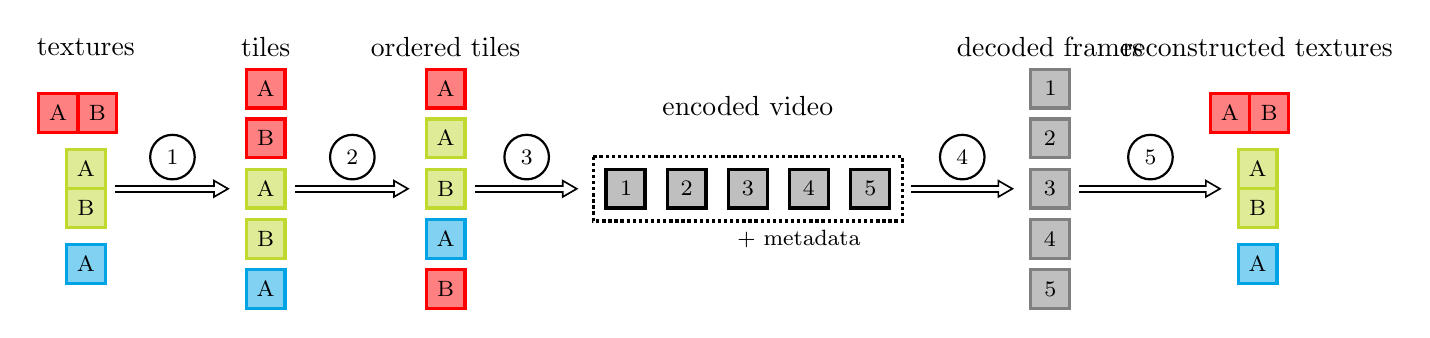
\begin{tikzpicture}[font=\footnotesize]

\def\wid{12}  
\def\hei{14}
\def\grad{50}
\def\ecart{-1pt}
\def\sizY{18pt}
\def\initial{-15pt}

\def\ecartYTexture{5pt}

\def\ecartXStep{65pt}

\tikzset{
textureUnit/.style={
    very thick,
    minimum height=\hei,
    text width = \wid,
    align = center,
    inner sep=1pt
    }
}

% ================================


\node[textureUnit, 
    fill=AdobeRed!\grad,
    draw = AdobeRed] (redA) {A};
\node[textureUnit,
    fill=AdobeRed!\grad,
    draw = AdobeRed,
    right=\ecart of redA] (redB) {B};

\node[textureUnit,
    fill=AdobeGreen!\grad,
    draw = AdobeGreen,
    xshift = 10pt,
    below = \ecartYTexture of redA] (greenA) {A};
\node[textureUnit,
    fill=AdobeGreen!\grad,
    draw = AdobeGreen,
    below=\ecart of greenA] (greenB) {B};

\node[textureUnit,
    fill=AdobeBlue!\grad,
    draw = AdobeBlue,
    below = \ecartYTexture of greenB] (blueA) {A};
    
\node[above=30pt of greenA, font=\normalsize] 
    (texture){textures};

% ================================

\node[textureUnit, 
    fill=AdobeGreen!\grad,
    draw = AdobeGreen]
    at ([xshift=\ecartXStep,yshift=7pt]greenB) (greenAextracted) {A};

\foreach \col/\letter/\i in {
    AdobeRed/A/2,
    AdobeRed/B/1}{
    \node[textureUnit,
        fill = \col!\grad,
        draw = \col,
        above=\initial + (\i*\sizY) of greenAextracted] 
        (\col\letter extracted) {\letter};
}    
    
\foreach \col/\letter/\i in {    
    AdobeGreen/B/1,
    AdobeBlue/A/2}{
    \node[textureUnit,
        fill = \col!\grad,
        draw = \col,
        below=\initial + (\i*\sizY) of greenAextracted] 
        (\col\letter extracted) {\letter};
}

\node[font=\normalsize] at (greenAextracted |- texture) {tiles};

% ================================

\node[textureUnit, 
    fill=AdobeGreen!\grad,
    draw = AdobeGreen]
    at ([xshift=\ecartXStep]greenAextracted) (greenAsequenced) {B};

\foreach \col/\letter/\i in {
    AdobeRed/A/2,
    AdobeGreen/A/1}{
    \node[textureUnit,
        fill = \col!\grad,
        draw = \col,
        above=\initial + (\i*\sizY) of greenAsequenced] 
        (\col\letter sequenced) {\letter};
}    
    
\foreach \col/\letter/\i in {    
    AdobeRed/B/2,
    AdobeBlue/A/1}{
    \node[textureUnit,
        fill = \col!\grad,
        draw = \col,
        below=\initial + (\i*\sizY) of greenAsequenced] 
        (\col\letter sequenced) {\letter};
}

\node[font=\normalsize] at (greenAsequenced |- texture) {ordered tiles};


% ================================

\node[textureUnit,
    fill=gray!\grad,
    draw=black]
    at ([xshift=\ecartXStep]greenAsequenced) (frameOne) {1};
    
\foreach \i in {2,...,5}{
    \node[textureUnit,
    fill=gray!\grad,
    draw=black]
    at ([xshift=(-1.3+1.3*\i)*17pt]frameOne) (na) {\i};}
    
\node[anchor=east] at ([yshift=-18pt]na)(metadata) {+ metadata};
\node[font=\normalsize] at ([yshift=30pt]$(frameOne)!0.5!(na)$) {encoded video}; 
    
\draw[very thick, densely dotted] 
    ([xshift=-4pt, yshift=4pt]frameOne.north west) rectangle 
    ([xshift=4pt, yshift=-4pt]na.south east);

% ================================

\node[textureUnit, 
    fill=gray!\grad,
    draw = gray]
    at ([xshift=\ecartXStep]na) (grayExtracted) {3};

\foreach \col/\letter/\i in {
    gray/1/2,
    gray/2/1}{
    \node[textureUnit,
        fill = \col!\grad,
        draw = \col,
        above=\initial + (\i*\sizY) of grayExtracted] 
        {\letter};
}    
    
\foreach \col/\letter/\i in {    
    gray/4/1,
    gray/5/2}{
    \node[textureUnit,
        fill = \col!\grad,
        draw = \col,
        below=\initial + (\i*\sizY) of grayExtracted] 
        {\letter};
}

\node[font=\normalsize] at (grayExtracted |- texture) {decoded frames};

    
% ================================

% \node[textureUnit, 
%     fill=AdobeGreen!\grad,
%     draw = AdobeGreen]
%     at ([xshift=\ecartXStep]grayExtracted) (greenAdecoded) {B};

% \foreach \col/\letter/\i in {
%     AdobeRed/A/2,
%     AdobeRed/B/-2}{
%     \node[textureUnit,
%         fill = \col!\grad,
%         draw = \col,
%         above=\initial + (\i*\sizY) of greenAdecoded] 
%         (\col\letter decoded) {\letter};
% }    
    
% \foreach \col/\letter/\i in {    
%     AdobeGreen/A/1,
%     AdobeBlue/A/-1}{
%     \node[textureUnit,
%         fill = \col!\grad,
%         draw = \col,
%         below=\i*\sizY of greenAdecoded] 
%         (\col\letter decoded) {\letter};
% }

\node[textureUnit, 
    fill=AdobeRed!\grad,
    draw = AdobeRed] 
    at ([xshift=\ecartXStep]grayExtracted |- redA) (redAdecoded) {A};
\node[textureUnit,
    fill=AdobeRed!\grad,
    draw = AdobeRed,
    right=\ecart of redAdecoded] (redBdecoded) {B};

\node[textureUnit,
    fill=AdobeGreen!\grad,
    draw = AdobeGreen,
    xshift=10pt,
    below = \ecartYTexture of redAdecoded] (greenAdecoded) {A};
\node[textureUnit,
    fill=AdobeGreen!\grad,
    draw = AdobeGreen,
    below=\ecart of greenAdecoded] (greenBdecoded) {B};

\node[textureUnit,
    fill=AdobeBlue!\grad,
    draw = AdobeBlue,
    below = \ecartYTexture of greenBdecoded] (blueAdecoded) {A};

\node[font=\normalsize] at (greenAdecoded |- texture) {reconstructed textures};


% ================================
\tikzstyle{vecArrow} = [thick, decoration={markings,mark=at position
   1 with {\arrow[semithick]{open triangle 60}}},
   double distance=1.4pt, shorten >= 5.5pt,
   preaction = {decorate},
   postaction = {draw,line width=1.4pt, white,shorten >= 4.5pt}]


\draw[vecArrow] ([xshift=3pt,yshift=7pt]greenB.east) to 
    node[above=3pt,circle,thick,draw] {1}
    ([xshift=-13pt]greenAextracted);
    
\draw[vecArrow] ([xshift=3pt]greenAextracted.east) to 
    node[above=3pt,circle,thick,draw] {2}
    ([xshift=-13pt]greenAsequenced);

\draw[vecArrow] ([xshift=3pt]greenAsequenced.east) to 
    node[above=3pt,circle,thick,draw] {3}
    ([xshift=-17pt]frameOne);
    
\draw[vecArrow] ([xshift=7pt]na.east) to 
    node[above=3pt,circle,thick,draw] {4}
    ([xshift=-13pt]grayExtracted);

\draw[vecArrow] ([xshift=3pt]grayExtracted.east) to 
    node[above=3pt,circle,thick,draw] {5}
    ([xshift=-13pt,yshift=7pt]greenBdecoded);
    

\end{tikzpicture}
\caption{Delivery chain: the different modules at the server side are \nod{1} tiling, then \nod{2} sorting, and then \nod{3} encoding; while the operations  at the client side are \nod{4} decoding and \nod{5} reconstructing.} \label{fig:system}
\end{figure*}

We propose to build a video from the set of textures that have to be delivered in a 3D multimedia application. Indeed, we observe that, in a large 3D scene, many textures have similarities, for example, multiple wood-based textures in a forest scene or marble-based textures in a palace. A video encoder can exploit this similarity between two independent textures in order to transmit both textures into a video of two frames where the first fame is the first texture and the second frame is what is needed to reconstruct the second texture from the information of the first frame.
Our proposal is illustrated in \Cref{fig:system}. We describe each of the steps in the following.

\subsection{At the Server Side}

The service provider prepares the sequence of images that is the input of the video encoder. We denote by $\mathcal T$ the set of textures that have to be delivered. The output at the server side is a video containing the data of $\mathcal T$ with as few losses as possible.

\newparag{Image Size Homogenization} All texture images in $\mathcal T$ do not have the same size, although the input of a video should have the same resolution. To homogenize the input of the video, our first operation (which is noted as \nod{1} in \Cref{fig:system}), is to cut each texture in $\mathcal T$ into unit \emph{texture tiled images}. In our example, both red and green textures are cut into two tiles that have the size of the smallest texture image. The resulting set of texture tiled images is noted $T$.

\newparag{Image Sequence Ordering} All texture tiled images in $T$ are then sorted based on their similarities. Let $d_{i,j}$ be the dissimilarity between two independent texture tiled images $i$ and $j$ in $T$. The lower is $d_{i,j}$, the more similar are $i$ and $j$. Our goal is to ensure that consecutive images have a high similarity, so that the video encoder can exploit this similarity and thus efficiently compress the video. The theoretical optimal solution of the sequence ordering is obtained by computing the minimum salesman traveling given the distance matrix $\mathcal D= \{d_{i,j}, \forall i,j \in T\}$. Indeed, the solution maximizes the sum of the similarities between every pair of consecutive images and includes all texture tiled images in the ordered sequence. The operation \nod{2} in \Cref{fig:system} results in a sequence noted $S$ that includes the whole set of information that is necessary to reconstruct $\mathcal T$.

\newparag{Video Encoding} The video encoder takes $S$ as input and builds a video that contains all tiled images (operation \nod{3} in \Cref{fig:system}). The main parameters that modern encoders require include the \emph{number of frames per second}, denoted by $f$, and the \emph{target video bit-rate}, denoted by $v$. Frames have no temporal relation, so the service provider can freely choose any value for $f$; the higher is $f$, the more texture tiled images are sent per time unit. However, since the number of texture tiled images to deliver is fixed, the settings of $f$ is linearly related to the video duration. For a sequence $S$ containing \num{300} images, a setting $f=30$ results in a video that is \SI{10}{\second} long. Then, for a given parameter $f$, the video bit-rate $v$ enables the settings of the quality; the higher is $v$, the lower is the compression and thus the higher is the quality of the images. Both parameters $f$ and $v$ allow the service provider to prepare multiple versions of the same set of textures $\mathcal T$, which can have multiple delivery delay and multiple qualities. Examples are given in \Cref{sec:performance}. 

\subsection{At the client side}

\newparag{Video Decoding} The client obtains the video and the set of metadata that enables the reconstruction of the texture images. It decodes the video and extracts a sequence $\Sigma$ of \emph{video frames}. This operation, noted \nod{4} in \Cref{fig:system}, is typically done in the \gls{GPU} of the client device. A major advantage of our solution is that the devices that can process 3D data to build a scene can also decode video in the most recent compression formats. Hence, our solution respects the universality feature of a texture delivery system.

\newparag{Texture Reconstruction} From the metadata file, the client is able to reconstruct the textures by appropriately stitching the decoded frames in $\Sigma$. The resulting set of textures $\mathcal R$ is a lossy version of the original set of textures $\mathcal T$ where the loss depends on the settings of both $f$ and $v$.

% -------------------------------------------------------
\section{Performance Evaluation}
\label{sec:performance}

We present here the result of a proof-of-concept experiment that we conducted to evaluate the potential of this idea. We used the well-known \emph{Viking Village} scene from \emph{Unity} Asset Store since it is a popular scene with high-quality textures and a reasonably large diversity of textures. The total size of all texture images is \SI{1.2}{\giga Bytes}. To manipulate smaller sets, we extracted a randomly selected set of \num{64} textures representing \SI{300}{\mega Bytes}.
 Since the height and width of the original texture images range from \num{256} to \num{4096}, we used a unit tile size of $\num{256}\times\num{256}$. We compute the dissimilarity between every pair of texture tiled images by using the \gls{MAE}. We used the \gls{HEVC} software from the \emph{libx265} library. The parameters are given in \Cref{tab:videos}. Finally, we computed the \gls{PSNR} between the original uncompressed texture images in $\mathcal T$ and the reconstructed images in $\mathcal R$.

\begin{table}[h]
\centering
\footnotesize
%\normalsize
\begin{tabular}{llll}
\toprule
\textbf{fps} & \textbf{length} & \textbf{bit-rate (in kilobits per s)} & \textbf{size (in megabytes)} \\
\midrule
2 & \SI{1566}{\second} & from \SI{50}{\kilo bps} to \SI{1250}{\kilo bps} & from \SI{9}{\mega B} to \SI{146}{\mega B}\\
60 & \SI{52}{\second}  & from \SI{5}{\mega bps} to {15}{\mega bps} & from \SI{31}{\mega B} to \SI{83}{\mega B}\\
120 & \SI{26}{\second} & from \SI{20}{\mega bps} to {40}{\mega bps} & from \SI{57}{\mega B} to \SI{101}{\mega B}\\
\bottomrule
\end{tabular}
\caption{Video settings and resulting size }\label{tab:videos}
\end{table}

To compare the performance of our solution with respect to state-of-the-art, we compressed the textures in $\mathcal T$ using both \emph{jpeg} and \emph{webp} from \emph{openCV}. We measured for both sets of compressed images the \gls{PSNR} and rate. The traditional rate-distortion curve is presented in \Cref{fig:rd} where the $y$-axis is the median \gls{PSNR} across all textures in $\mathcal R$.

\begin{figure}[h]
\centering
\begin{tikzpicture}
\begin{axis}[
   ylabel = median PSNR (dB), ymin =30, ymax=60,
   xlabel = bytes per pixel, xmin=0, xmax=1,
   height = 35ex,
   width=\columnwidth,
   legend pos = south east,
   %legend columns = 2,
   legend cell align = left,
   legend style = {
    %  at = {(0.5,1.03)},
    %  anchor = south,
      draw = none,
      font=\footnotesize,
   },
   cycle list name=adobe-rd,
   ]

   \addplot+ %[error bars/.cd,
             %  y dir=both, y explicit]
             table[
               x=rate,
               y=mean_dist,
             %  y error plus = max_dist,
             %  y error minus = min_dist,
            ] {CSV_for_RD/rd_optimalSequence.csv};
   \addlegendentry{video}
  
   \addplot+ %[error bars/.cd,
             %  y dir=both, y explicit]
             table[
               x=rate,
               y=mean_dist,
             %  y error plus = max_dist,
             %  y error minus = min_dist,
            ] {CSV_for_RD/rd_jpg.csv};
   \addlegendentry{jpeg}

   \addplot+ %[error bars/.cd,
             %  y dir=both, y explicit]
             table[
               x=rate,
               y=mean_dist,
             %  y error plus = max_dist,
             %  y error minus = min_dist,
            ] {CSV_for_RD/rd_webp.csv};
   \addlegendentry{webp}

\end{axis}
\end{tikzpicture}
\caption{Rate-distortion}\label{fig:rd}
\end{figure}


Although we show the result of our earliest experiments without any additional optimization, our approach using video encoder has compression performance that is at least as good as the state-of-the-art \emph{webp} image compression library. The main advantage of our approach is that we have a wider range of settings that are possible, and thus we able to provide a solution that is more adaptive. Furthermore, we have a larger set of options, including more qualitative compression of textures.

% -------------------------------------------------------
\section{Research Opportunities}
\label{sec:conclusion}

We have introduced in this paper a new approach to deliver a set of textures by encoding them into a video. We highlighted themain features of this approach: $(i)$ its legacy to existing delivery software and hardware, and $(ii)$ its better adaptivity to client resources, including more delivery options at high quality. This paper describes our earliest work in this area. Many research questions are still open, including $(i)$ The video decoding is processed in the \gls{GPU}. Since 3D scene processing is also done in the \gls{GPU}, it is possible to design a pipeline between the video decoder and the 3D engine in order to bypass the traditional \gls{GPU} I/O bottleneck. $(ii)$ video compression with \gls{HEVC} is more effective with larger frames. The tiling operation could be improved in order to put larger input images to the video encoder. $(iii)$ Textures may have different format and structures (albedo, mask, depth map). Instead of having only one sequence of textures, we can create subsets of textures from their similarities. $(iv)$ optimization problems should be studied to find the trade-off between quality, delay, and resource usages with respect to the distance of the camera to the texture and to the object on which the texture applies. The solution that we introduced in this paper opens multiple exciting research opportunities with potentially high rewarding benefits for the delivery problem in the 3D multimedia application.


\bibliographystyle{abbrv}

\bibliography{biblio.bib}
\end{document}
